\documentclass[11pt,a4paper]{article}
\usepackage[utf8]{inputenc}
\usepackage[spanish]{babel}
\usepackage{amsmath}
\usepackage{graphicx}
\usepackage{color}
\usepackage{amsfonts}
\usepackage{amssymb}
\begin{document}

\begin{center}

\textcolor{blue}{Universidad de Guanajuato}\\
Geometría Computacional\\
\begin{large}
Proyecto Final\\

\end{large}
Profesora: Lizárraga Morales Rocío Alfonsina\\
17/12/2020\\
\rule{70mm}{.1mm}\\
\bf{Emmanuel Alejandro Gallardo Domínguez}\\
\bf{Guadalupe Carolina Aguirre Zúñiga}\\
145884\\

\end{center}


\begin{center}

\bf{{\huge Nenúfares - Monet}}
\end{center}

\section{Resumen:}
En este proyecto se analizó una obra del reconocido pintor Claude Monet, nenúfares (o mejor conocida como Japanese Bridge) para ser reinterpretada y convertida a una pieza digital con toques de aleatoriedad y geometría computacional.
\section{Introducción}
% Contextualización de la propuesta, justificación, propuesta
	Como propuesta de proyecto se eligió la opción de reinterpretar una obra y convertirla en una obra en digital.\\
	Claude Monet fue uno de los pioneros en el impresionismo, estilo artístico que ejecutaría toda su vida. Esta obra nos llamó mucho la atención por varios motivos:	
	
	\subsection{Los colores a usar: }
		\begin{center}
			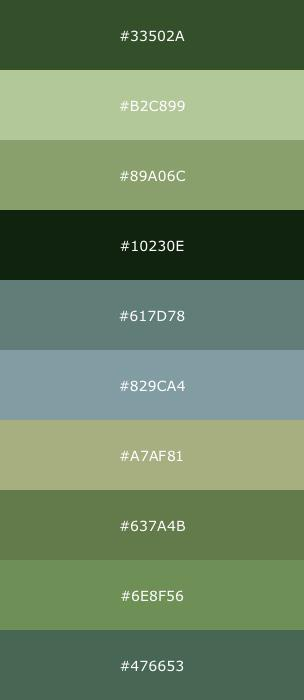
\includegraphics[scale=.3]{PaletaDeColores}
		\end{center}
			Son colores que pueden ser interpretados como "Verde, naturaleza", siempre presentes en los colores, de nuestra 	opinión, más neutrales y llamativos.
	\subsection{Los elementos que posee:}
		Al ser una representación de la naturaleza podíamos jugar con la aleatoriedad de esta, generando partes del terreno con funciones nativas de processing como veremos más adelante
	\subsection{El reto que implicaba: }
		Se asumió que la reinterpretación de una obra de impresionismo sería un buen reto técnico, por los colores, por la correcta colocación de los objetos o hasta por la programación de los mismos.

\section{Metodología}
	Para poder describir mejor el funcionamiento diseñado para este proyecto es útil dividirlo en dos diferentes tipos de módilos/objetos creados:
	\begin{itemize}
	\item {\bf Objetos:} Podemos llamarles de esta forma a los módulos que son visibles en el programa, y que si bien tienen su parte de back end al ser generados, en su mayor parte se usan como decorativos.
	\item { \bf Auxiliares: } Se trata de módulos que fueron implementados para incrementar la funcionalidad y a pesar de no ser visibles, hacen del programa cómodo de usar
	\end{itemize}
	\subsection{Objetos: }
		\subsubsection{\textcolor{blue}{Estanque}}
			Se trata de un objeto tridimensional que genera un mapa de ruido aleatorio usando la función \textcolor{red}{noise()} de Processing. 

			\begin{center}
			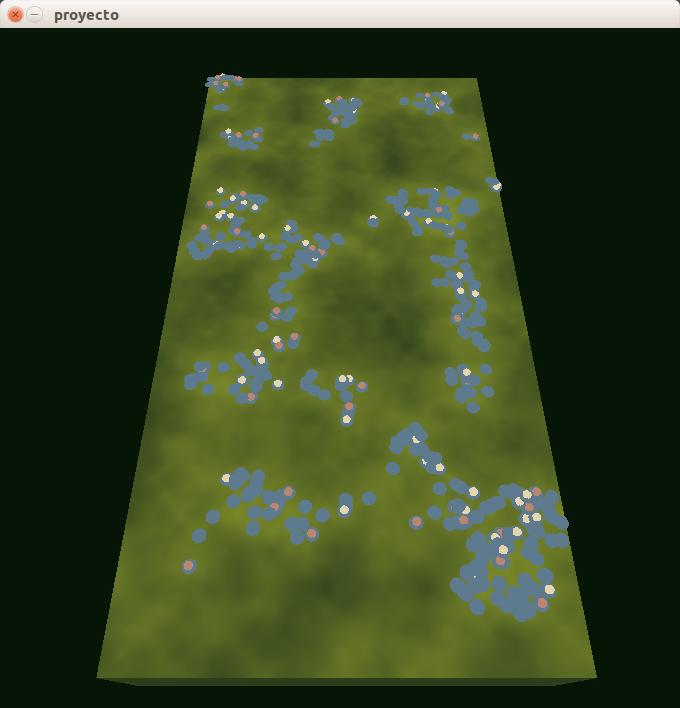
\includegraphics[scale=.5]{CAP1}
			\end{center}




\section{Resultados}
\section{Conclusiones}
\section{Bibliografía}


 	
\end{document}